\documentclass[11pt]{article}
\usepackage[a4paper,margin=0.88in]{geometry}
\usepackage[T1]{fontenc}
\usepackage[utf8]{inputenc}
\usepackage{lmodern}
\usepackage{amsmath,amssymb,booktabs,graphicx,url,hyperref,array,microtype}
\usepackage{caption}
\hypersetup{colorlinks=true,linkcolor=black,citecolor=blue,urlcolor=blue}
\setlength{\columnsep}{0.24in}
\title{Uncertainty-Guided Oracle Verification for Scientific Citation-Intent Labelling: A Controlled Comparison on SciCite}
\author{Ujjwal Nikam\\IIIT Allahabad}
\date{}
\begin{document}
\maketitle
\begin{abstract}
Scientific text annotations can contain errors even when generated by competent classifiers. We investigate whether ranking predictions by uncertainty makes a limited verification budget more effective than randomly choosing predictions for review. On the SciCite citation-intent dataset, we train TF--IDF logistic regression and linear SVM baselines and simulate corrections using reference labels. On 914 validation examples after removing two exact train--validation text overlaps, the SVM attains 82.82\% accuracy and 0.8022 macro-F1. At a budget of 100 corrected instances, uncertainty-guided oracle verification yields 87.53\% validation accuracy, compared with 84.66\% mean accuracy for random verification over 100 repeats. On the 1,859-instance held-out test set, the corresponding accuracies are 85.10\%, 83.24\%, and 82.30\% for uncertainty-guided, random, and uncorrected SVM predictions. Filtering out test instances associated with citing papers occurring in training preserves the pattern on 1,624 examples. The experiment shows that low-margin examples concentrate model errors under this setup; since corrections are simulated with reference labels, it does not demonstrate human review accuracy, time savings, or causal effects of AI suggestions on annotators.
\end{abstract}
\noindent\textbf{Keywords:} scientific text annotation; citation intent; uncertainty sampling; human-in-the-loop; reproducible evaluation; label quality.

\section{Introduction}
Machine-learning research depends on reference labels that are costly to generate and not necessarily free of mistakes. Prior comparisons of language-model-assisted labelling and human annotation report task-dependent trade-offs in quality and throughput \cite{gilardi2023chatgpt,turner2025large,chen2025human}. Other work identifies label noise in established benchmarks \cite{northcutt2021pervasive}, while active learning motivates focusing annotation effort on uncertain inputs \cite{settles2009active}. These observations motivated our prior review of manual, automated and hybrid scientific annotation pipelines.

The practical problem considered here is not whether a model can replace human experts. Given a fixed number of predictions that could be reviewed, \emph{which predictions should be selected?} We compare two transparent selection policies, random selection and low decision-score margin, under equal review budgets. Our study intentionally uses perfect reference-label substitution as an \emph{oracle simulation}, isolating the value of case selection from human reviewer errors. It thus estimates an attainable upper-bound correction outcome, not operational performance of actual annotators.

The contributions of this course-level controlled study are: (i) a common-protocol comparison of inexpensive citation-intent classifiers; (ii) measured budget--accuracy and budget--error-recovery curves; (iii) a held-out test at a selected review budget; and (iv) a sensitivity analysis for shared citing papers. We do not claim to introduce a new sampling algorithm or novel model.

\section{Related Work and Research Question}
Cohan et al. introduced the SciCite citation-intent corpus with three citation-function labels and methods for classifying scientific citation context \cite{cohan2019structural}. Their neural scaffold approach is part of the dataset's original work; our TF--IDF baselines are separate, lightweight comparators, not faithful reproductions of their original model.

Active-learning literature describes uncertainty-based sampling as a way of choosing informative examples \cite{settles2009active}. Our experiment instead uses a \emph{fixed pretrained classifier} and selects its predictions for simulated correction; it does not update the classifier after acquiring new labels. This distinction matters: a correction queue can improve a delivered annotation collection without necessarily improving the underlying trained model.

Studies of AI-assisted annotation suggest that hybrid pipelines can benefit from machine-generated proposals while remaining vulnerable to unchecked errors and reviewer behavior \cite{chen2025human,dreizin2023accelerating}. We therefore restrict our claim to the testable computational question:

\emph{RQ1: For SciCite citation-intent labels, does selecting the lowest-margin SVM predictions recover more errors and improve final annotation accuracy more than random selection at the same correction budget?}

\emph{RQ2: Does the pattern remain on held-out test data and when examples sharing citing papers with training are excluded?}

\section{Dataset and Methods}
\subsection{Data and baseline models}
We use the three official SciCite splits: 8,194 unique-ID training records, 916 validation records and 1,859 test records. The text input is the JSONL \texttt{string} field; class targets are \texttt{background}, \texttt{method}, and \texttt{result}. Record-level deduplication by \texttt{unique\_id} leaves these split counts unchanged. There are no missing training texts in the recorded audit.

Each baseline uses TF--IDF with unigrams and bigrams, a vocabulary cap of 20,000, and default vectorizer settings. We fit logistic regression (\texttt{max\_iter=1000}, \texttt{random\_state=42}) and \texttt{LinearSVC} (\texttt{random\_state=42}) on the official training data. We evaluate accuracy and macro-averaged F1. These settings are shared where applicable, with library defaults otherwise, and the environment records Python 3.13.16, scikit-learn 1.6.1, NumPy 2.1.3 and pandas 2.2.3.

\subsection{Overlap controls}
Auditing exact citation text identifies one duplicated text within the training split, two texts shared between training and validation, and none shared between training and test. The validation comparison first includes the official 916 examples, then excludes the two cross-split text overlaps, yielding 914 for leakage-controlled reporting. The trained models are unchanged by this filtering. The audit also identifies 468 citing-paper IDs shared between train and validation, and 226 shared between train and test. These counts describe overlap in \emph{paper identifiers}, not numbers of overlapping test examples.

For a sensitivity analysis we filter the test examples by whether \texttt{citingPaperId} occurs in the training set; 235 test records are excluded, leaving 1,624. This is a post-hoc paper-disjoint \emph{evaluation subset}, not a fully rebuilt group-disjoint training/validation/test protocol.

\subsection{Uncertainty ranking and oracle correction}
The SVM outputs a vector of class decision scores $s(x)$. For each example we rank the scores and calculate the top-two margin
\begin{equation}\label{eq:margin}
 m(x)=s_{(1)}(x)-s_{(2)}(x),
\end{equation}
where $s_{(1)}\ge s_{(2)}$ denote the highest and second-highest score. Smaller margins define the uncertainty queue. Such scores are not calibrated class probabilities.

For a budget $b$, the uncertainty policy selects the $b$ smallest-margin examples; a random policy draws $b$ without replacement. Each selected prediction is replaced by its dataset reference label, whether or not it was initially correct. All unselected predictions remain unchanged. Hence, with $N$ examples and $e_b$ wrong predictions among selected records,
\begin{equation}\label{eq:accuracy}
 \mathrm{Accuracy}_{\mathrm{corrected}}=\mathrm{Accuracy}_{\mathrm{base}}+e_b/N.
\end{equation}
The protocol assumes flawless verification and makes no claim about human review behavior. Random policies use 100 iterations with NumPy seed 42; each uncertainty queue is deterministic on the fixed evaluation set.

\subsection{Experimental protocol}
Validation budgets are $b\in\{0,10,25,50,100,150,200,300\}$ on 914 records. These validation results inform the held-out study; the primary held-out comparison uses $b=100$ on 1,859 records, approximately 5.38\% of the test set. The sensitivity subset uses $b=87$ on 1,624 records, preserving approximately the same review fraction. Test-model weights and hyperparameters are not changed. We report random means and sample standard deviations across 100 draws; these are dispersion across simulated random queues, not confidence intervals over new datasets.

\section{Experimental Results}
\subsection{Classification baseline and errors}
Table~\ref{tab:baseline} summarizes the leakage-controlled validation baselines. Linear SVM has slightly higher scores; the difference does not by itself establish statistical superiority. Its official 916-example validation confusion matrix (Fig.~\ref{fig:cm}) contains 157 errors; most notably, 68 method examples are assigned to background, making method/background confusion a substantial failure mode.

\begin{table}[t]
\centering
\caption{Baseline results on 914 validation instances after excluding two exact training-text overlaps.}
\label{tab:baseline}
\begin{tabular}{lcc}\toprule
Model & Accuracy & Macro-F1\\\midrule
TF--IDF + logistic regression & 0.8271 & 0.7913\\
TF--IDF + linear SVM & \textbf{0.8282} & \textbf{0.8022}\\\bottomrule
\end{tabular}
\end{table}

\begin{figure}[t]
\centering
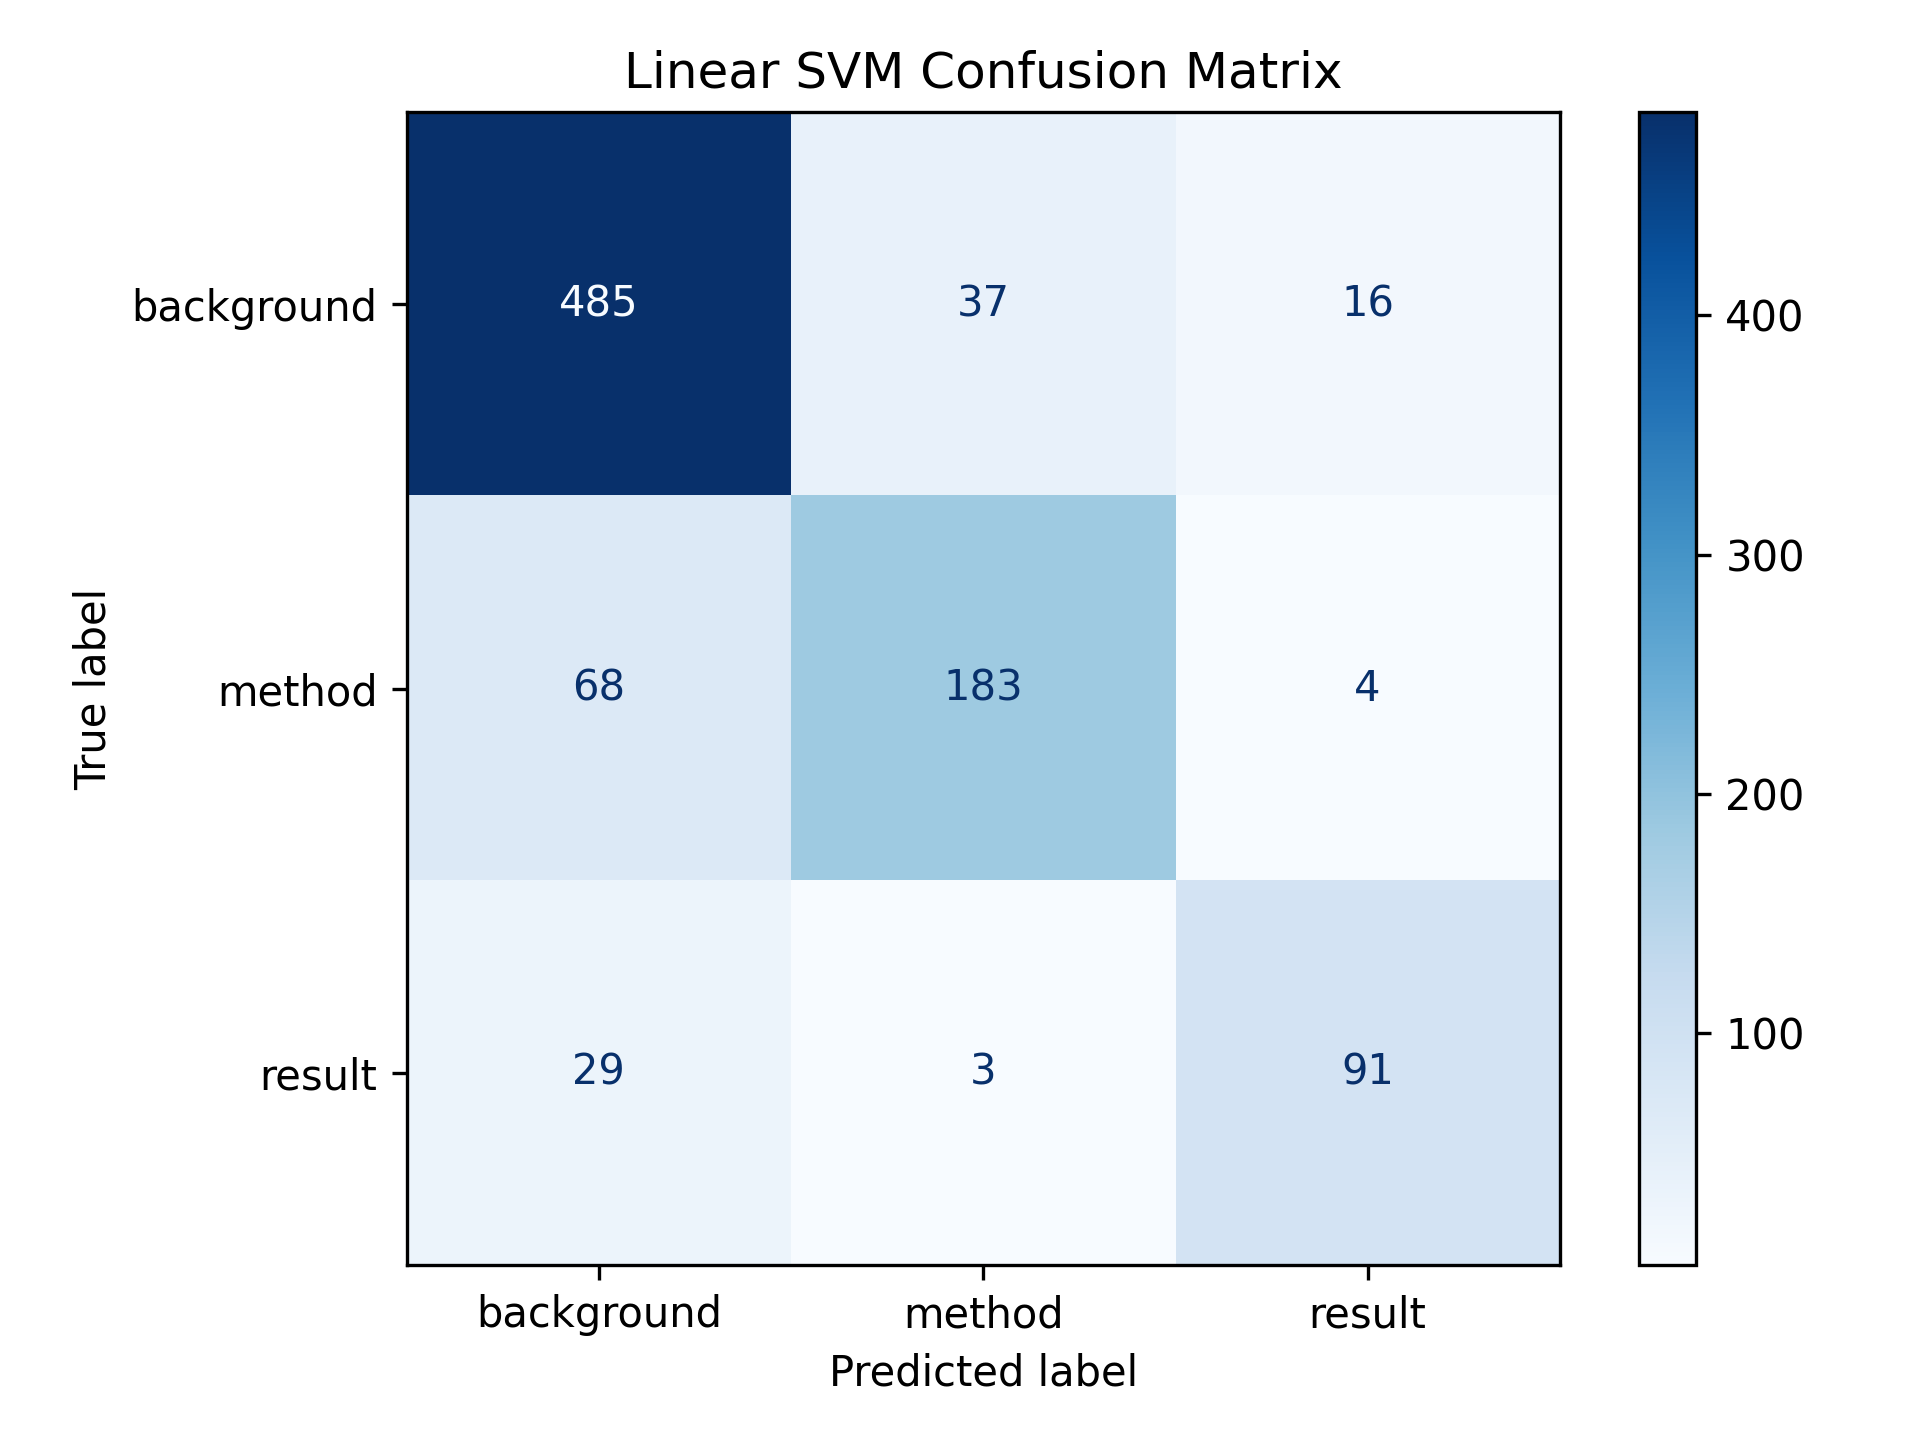
\includegraphics[width=\columnwidth]{figures/svm_confusion_matrix.png}
\caption{Linear SVM confusion matrix on the original 916-instance validation split. Rows are reference labels and columns are predictions. This figure predates exclusion of the two overlapping contexts; the principal metrics in Table~\ref{tab:baseline} use 914 instances.}
\label{fig:cm}
\end{figure}

\subsection{Validation correction efficiency}
Table~\ref{tab:validation} and Figures~\ref{fig:curve}--\ref{fig:errors} show the systematic validation-budget evaluation. At $b=100$, uncertainty-guided correction discovers 43 model errors compared with 16.83 errors on average for random selection, improving accuracy to 0.8753 versus 0.8466. At $b=300$, uncertainty correction identifies 101 errors compared with 52.35 on average for random selection. The evidence supports concentration of model mistakes in low-margin predictions for this dataset and classifier.

\begin{table}[t]
\centering
\caption{Validation correction accuracy (914 records). Random entries average 100 runs; uncertainty uses one deterministic margin ranking.}
\label{tab:validation}
\begin{tabular}{rcc}\toprule
Budget & Random mean & Uncertainty\\\midrule
0 & 0.8282 & 0.8282\\
25 & 0.8325 & 0.8392\\
50 & 0.8379 & 0.8512\\
100 & 0.8466 & 0.8753\\
150 & 0.8556 & 0.8972\\
200 & 0.8661 & 0.9147\\
300 & 0.8855 & 0.9387\\\bottomrule
\end{tabular}
\end{table}

\begin{figure}[t]
\centering
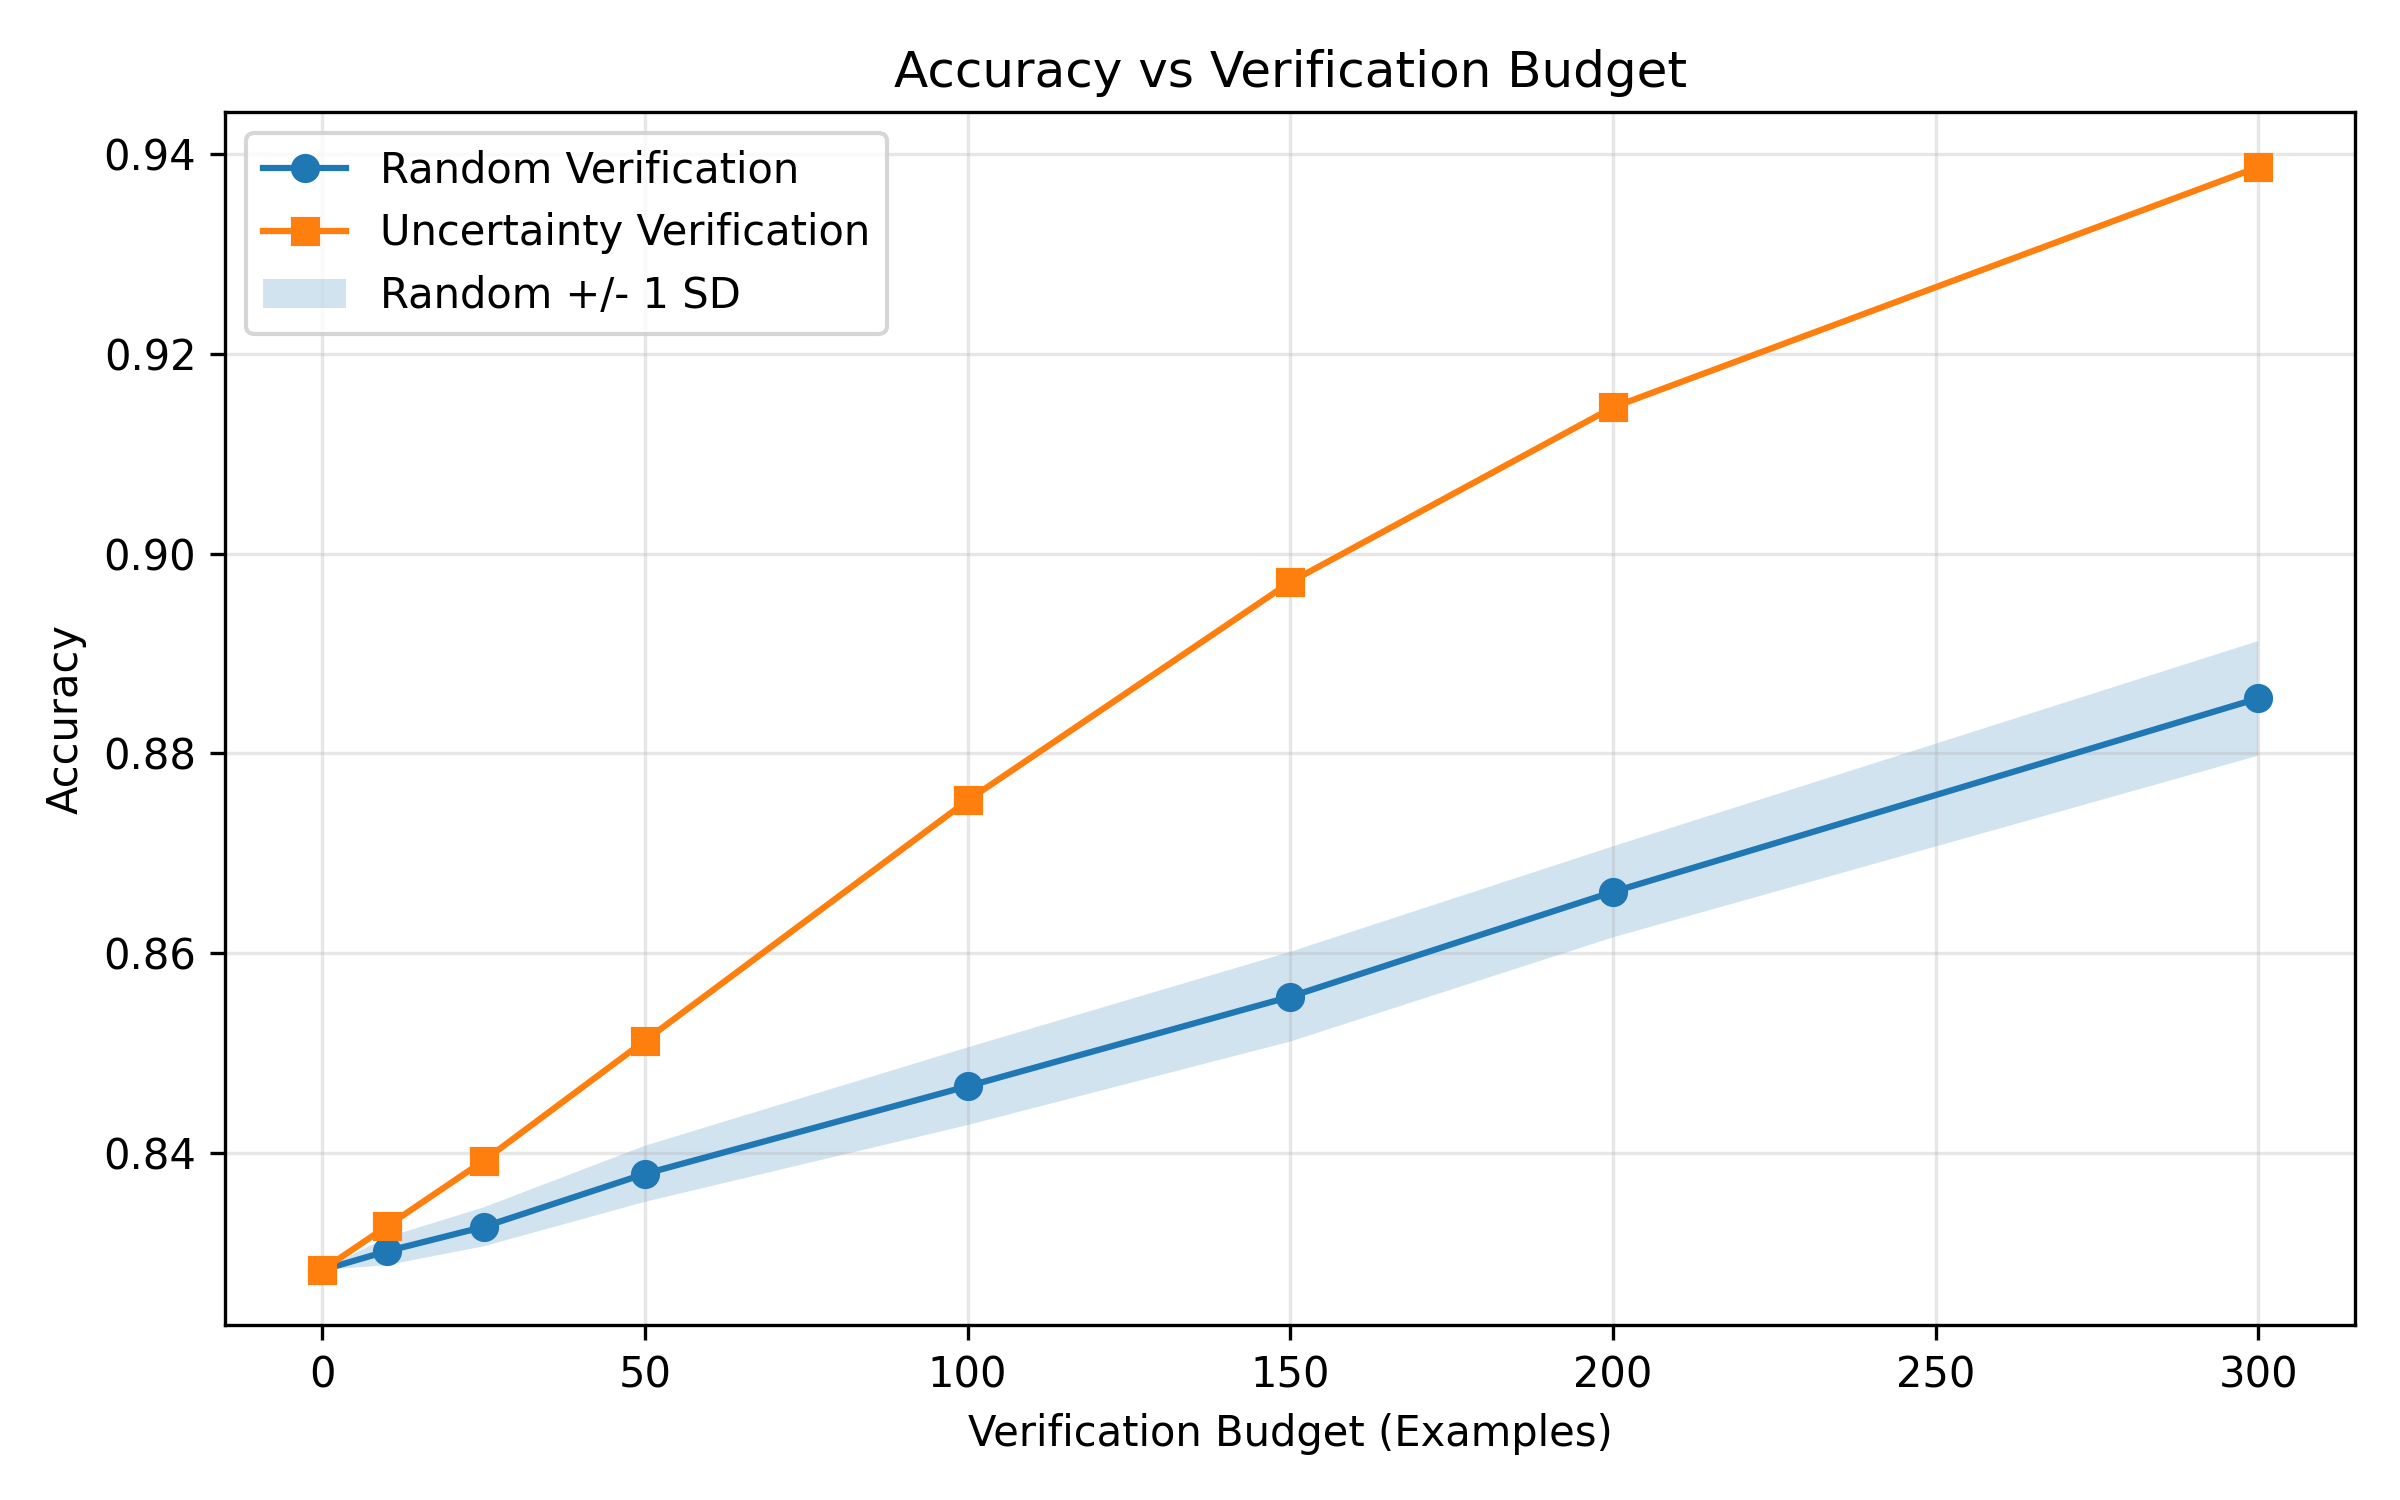
\includegraphics[width=\columnwidth]{figures/verification_accuracy_curve.png}
\caption{Validation accuracy as a function of number of perfect oracle corrections. The band is random-sampling mean $\pm$ one standard deviation across 100 runs, not a confidence interval.}
\label{fig:curve}
\end{figure}

\begin{figure}[t]
\centering
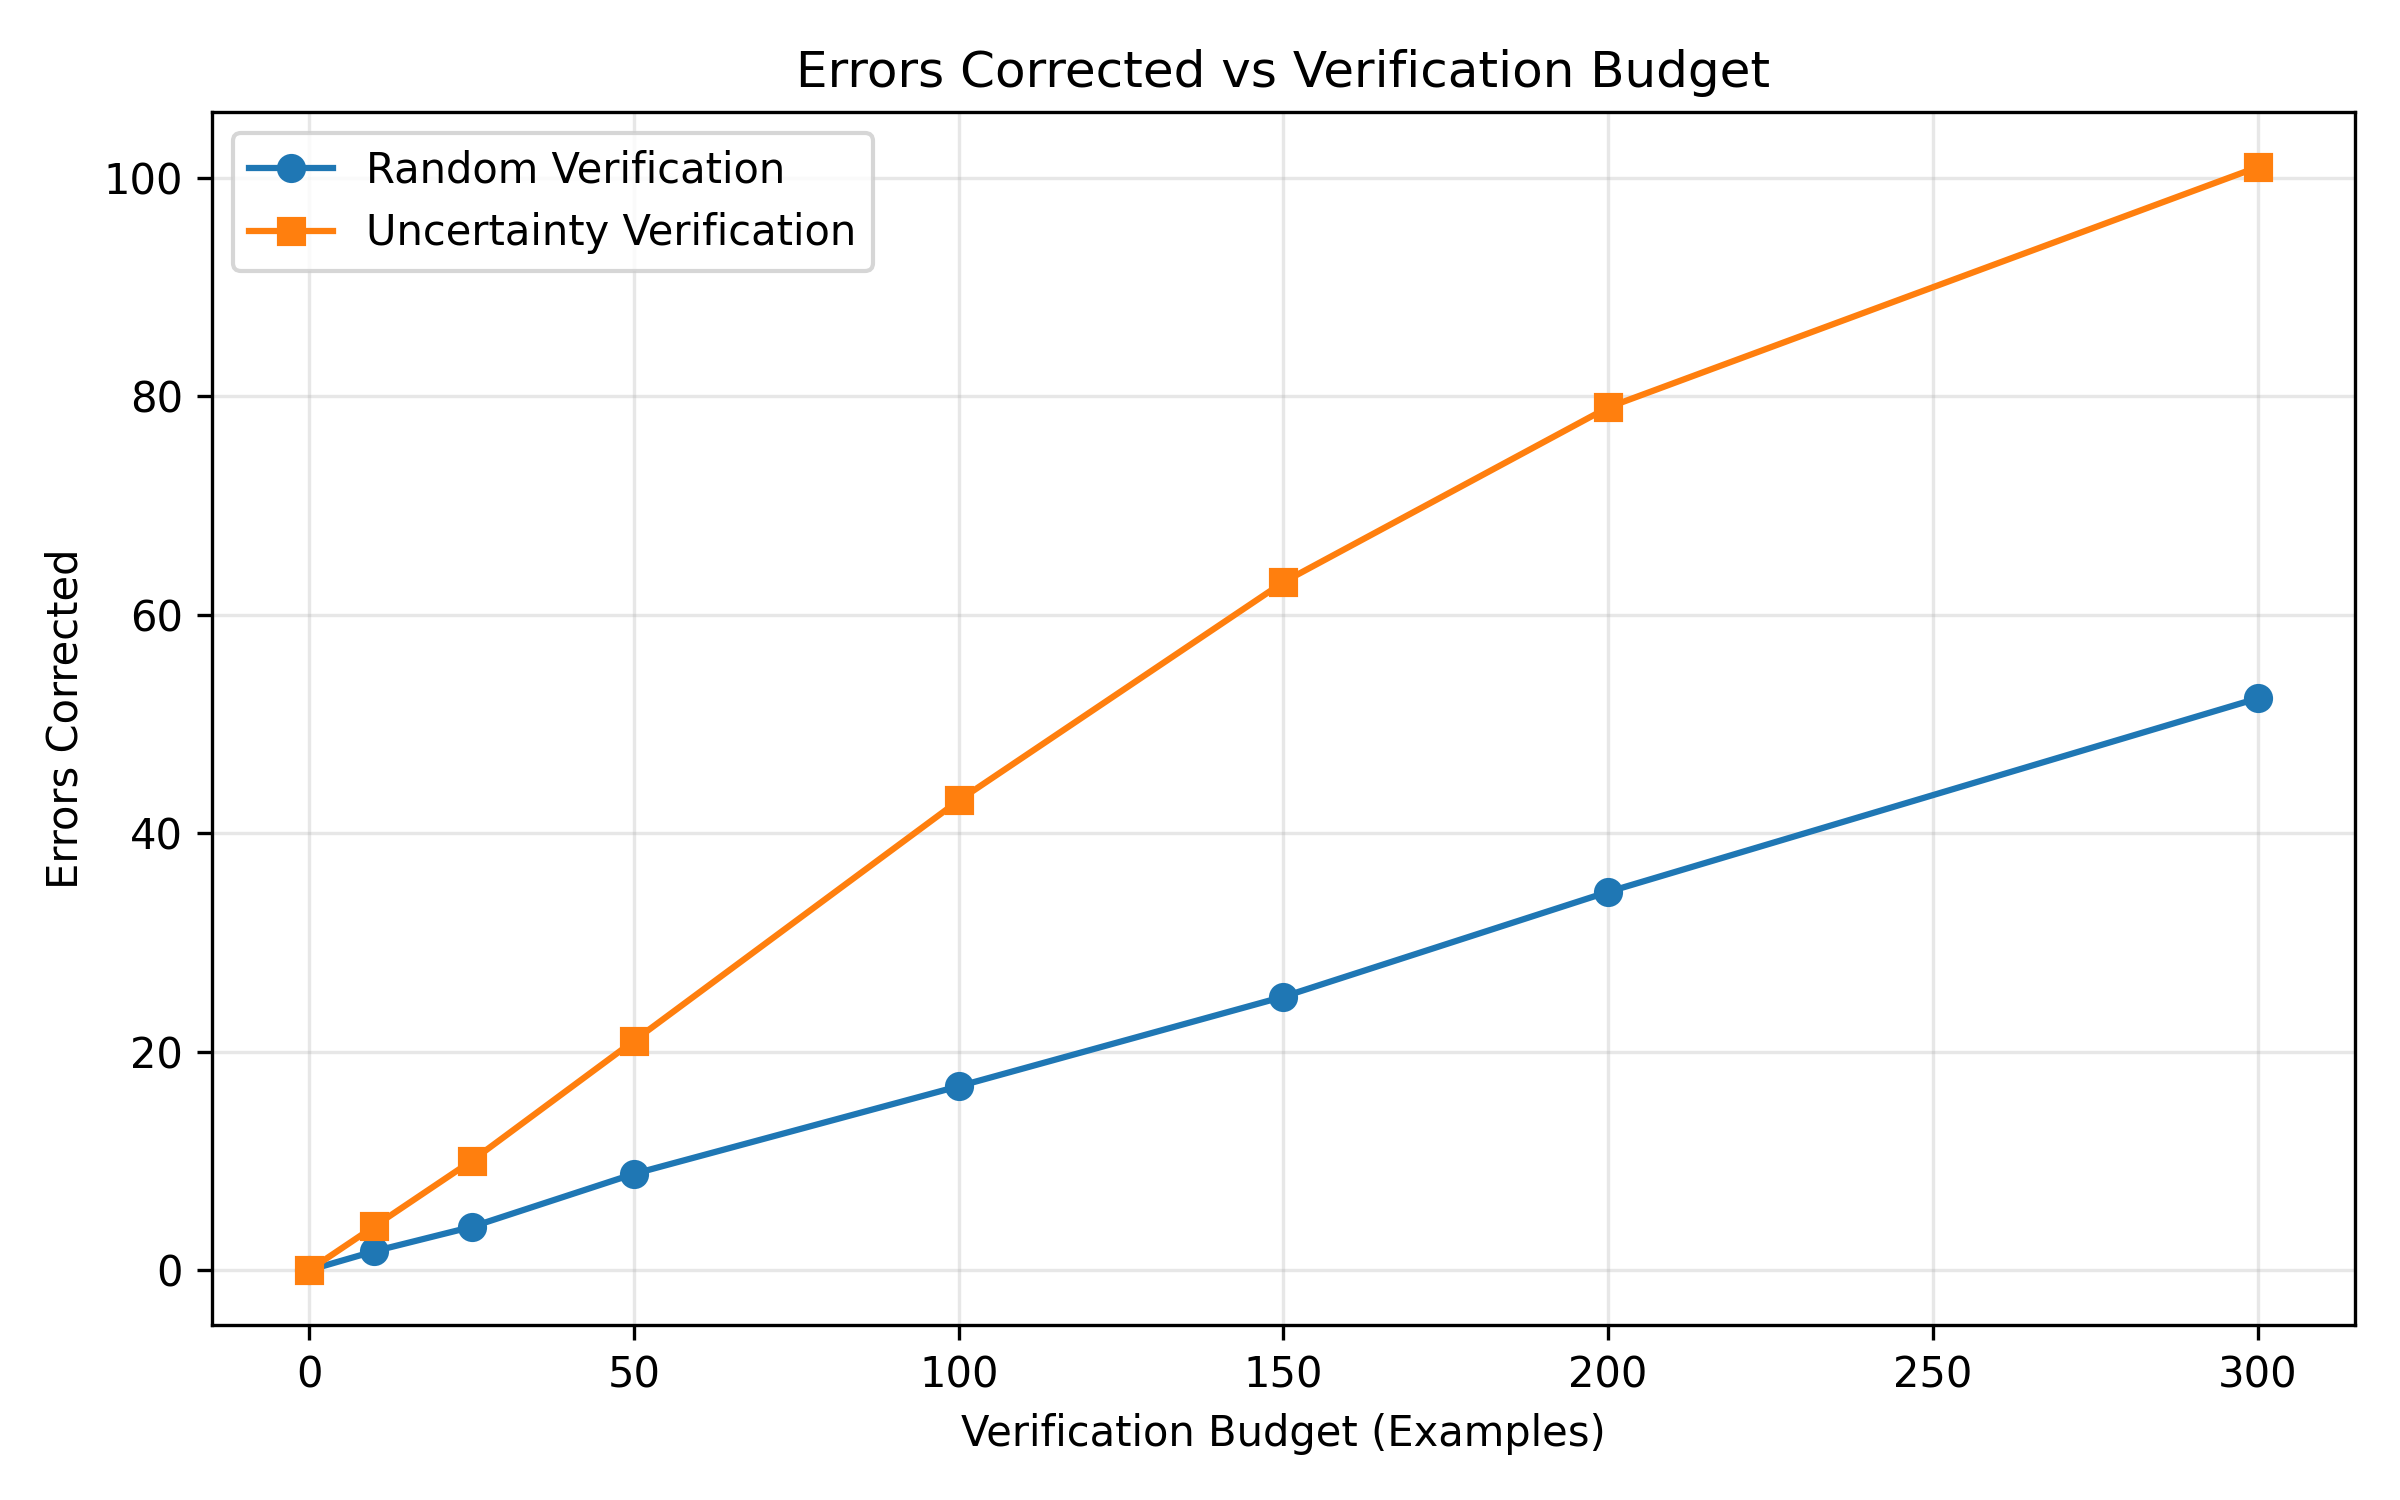
\includegraphics[width=\columnwidth]{figures/errors_corrected_curve.png}
\caption{Validation errors corrected versus fixed review budget. Errors are counted against dataset reference labels.}
\label{fig:errors}
\end{figure}

\subsection{Held-out evaluation and sensitivity analysis}
On the 1,859-example test set, the uncorrected SVM makes 329 errors and obtains 0.8230 accuracy and 0.8040 macro-F1. At $b=100$, low-margin selection locates 52 of those errors, yielding 0.8510 accuracy and 0.8349 macro-F1. Random selection produces 0.8324 mean accuracy (standard deviation 0.00216) and 0.8143 mean macro-F1. Table~\ref{tab:test} reports both this comparison and the paper-disjoint sensitivity analysis.

The paper-disjoint subset contains 1,624 examples; the classifier produces 298 incorrect labels before review. At $b=87$, uncertainty selection locates 43 wrong predictions and improves accuracy from 0.8165 to 0.8430. Random correction reaches 0.8266 on average. Both tests preserve the observed direction of the validation comparison, while the sizes and review budgets differ.

\begin{table*}[t]
\centering
\caption{Held-out test and filtered paper-disjoint subset. All corrections are perfect oracle substitutions. Random results are 100-run means; baseline and uncertainty results are deterministic.}
\label{tab:test}
\begin{tabular}{llrrrr}\toprule
Evaluation & Strategy & Examples & Review budget & Accuracy & Macro-F1\\\midrule
Held-out test & SVM baseline & 1859 & 0 & 0.8230 & 0.8040\\
 & Random & 1859 & 100 & 0.8324 & 0.8143\\
 & Uncertainty & 1859 & 100 & \textbf{0.8510} & \textbf{0.8349}\\\midrule
No shared citing paper with training & SVM baseline & 1624 & 0 & 0.8165 & 0.8050\\
 & Random & 1624 & 87 & 0.8266 & 0.8158\\
 & Uncertainty & 1624 & 87 & \textbf{0.8430} & \textbf{0.8331}\\\bottomrule
\end{tabular}
\end{table*}

\section{Discussion}
These outcomes are mechanically interpretable: margin ranking prioritizes borderline SVM decisions, which are often more likely to be wrong than high-margin predictions. On validation, 43 of the first 100 selected examples are actual errors; on held-out test, 52 of 100 are actual errors, versus 329 errors across all 1,859 test predictions. Consequently, the same correction budget addresses more wrong labels when focused by uncertainty. The improvement should not be interpreted as guaranteed across classifiers or disciplines.

The comparison illustrates two separate concepts. \emph{Selection efficiency} asks how well a ranking finds mistakes; \emph{verification fidelity} asks whether a reviewer correctly identifies and fixes them. Our design isolates selection efficiency by granting an oracle. A real human-in-the-loop workflow may exhibit disagreement, time costs, or automation bias \cite{chen2025human}; therefore, its measured benefit may be lower. Similarly, accuracy against dataset labels is meaningful only to the extent that those labels form a reliable reference \cite{northcutt2021confident,northcutt2021pervasive}.

The fixed held-out test budget of 100 was chosen after exploring budgets on validation, not preregistered prior to all work. We made no model modifications based on held-out performance. Because the held-out test was inspected in this completed study, further model or budget development should use a newly isolated evaluation set rather than treating these same test outcomes as fresh confirmatory evidence.

\section{Limitations and Threats to Validity}
\textbf{Reference-label dependence.} Oracle correction assumes SciCite labels are correct; our study did not independently adjudicate ambiguous citations. Dataset labels are not necessarily infallible.

\textbf{Human interpretation.} No annotators participated. There is no measured reviewer time, cost, behavioral bias, inter-rater reliability, or measured human verification accuracy. The study must not be presented as a human-subject experiment.

\textbf{Split dependence.} Two exact train--validation text overlaps were removed for primary validation reporting, but overlapping citing-paper IDs remain in the official splits. The paper-filtered evaluation excludes 235 test examples, but is not equivalent to retraining with wholly group-disjoint partitions. Source papers can be related even without matching identifiers.

\textbf{Generalization and method choices.} We use one scientific-text dataset and one principal uncertainty score, a fixed linear model, and a single classifier fit. We do not assess model-seed variability, calibrated uncertainty, transformer baselines, alternative scientific disciplines, or annotation cost. Standard deviations describe random selection only and do not by themselves establish population-level significance.

\textbf{Dataset and artifact provenance.} The exact dataset archive hash is recorded in the earlier environment test; raw data are not included in the public paper bundle. Its data reuse terms should be checked independently before redistribution. Notebook runs and CSV results provide primary evidence; the originally exported \texttt{experiment\_summary.json} contains a field-level reporting defect: \texttt{test\_baseline\_macro\_f1} incorrectly contains the paper-disjoint value 0.805048. The verified held-out test CSV gives 0.803991, which is used here. The underlying predictions and held-out CSV were not changed to repair this metadata issue.

\section{Reproducibility and AI-Assisted Workflow}
The notebook executes dataset loading, two baselines, validation confusion/error analysis, overlap auditing, low-margin scoring, random-versus-uncertainty correction simulation, held-out evaluation, and paper-disjoint sensitivity analysis. Key output CSVs and the generated plots are preserved in the evidence package. In particular, the test procedure fixes the SVM, review budget of 100, 100 random draws, and seed 42. The repository should include the original executed notebook, source data-acquisition instructions, scikit-learn and Python versions, the evidence files, and commands for a fresh rerun.

AI assistance was used to draft and debug code and help structure the experiment. Early data loaders incorrectly referred to a nonexistent \texttt{context} field, producing a \texttt{KeyError}; inspection of the actual JSONL schema established that \texttt{string} is the relevant field. Subsequent genuine Colab runs verified split counts and baselines. An additional reporting error in a JSON summary was found by cross-checking the exported CSVs. These corrections illustrate why proposed code and prose require human execution and independent validation rather than acceptance on appearance.

\section{Conclusion}
On SciCite citation-intent classification, ranking predictions by SVM top-two decision-score margin made a fixed budget of perfect oracle corrections more productive than random selection. At 100 held-out test reviews, the ranking identified 52 incorrect predictions and raised accuracy from 82.30\% to 85.10\%, compared with 83.24\% mean accuracy under random review. A filtered paper-disjoint subset preserved the same qualitative trend. These findings support the value of uncertainty as an error-triage signal within the specific tested pipeline, while leaving genuine human verification efficiency, broader generalization, and complete group-disjoint training for future experiments.

\bibliographystyle{plain}
\bibliography{references}
\end{document}
